\chapter[Van Dantzig Pairs and Transport]{Van Dantzig Pairs, Wald Couples and the Sine Squared Transport}\label{ch:10d}

In 1958 David van Dantzig posed a prize question in the Nieuw Archief voor Wiskunde \cite{vandantzig1958}: describe the characteristic functions $F$ for which $t\mapsto1/F(it)$ is again a characteristic function. The cosine and the hyperbolic secant form the simplest example, and Lukacs \cite{lukacs1968,lukacs1970} turned the question into a theory. Roynette and Yor \cite{roynetteyor2005} rewrote the Riemann hypothesis in terms of Wald couples and P\'olya frequency functions; the first author \cite{polson2018vdp} observed that the Hadamard factorisation of a Laguerre P\'olya function is the same thing as a van Dantzig pair, a Wald couple and a Thorin representation, three probabilistic readings of one product; and more than sixty years after the prize question Konstantopoulos, Patie and Sarkar \cite{konstantopoulospatiesarkar2024} showed that the Riemann hypothesis is a statement about the Lukacs subclass of van Dantzig's class. This chapter assembles these ideas for automorphic $L$ functions. We describe the van Dantzig problem and its Lukacs subclass, Wald couples and the duality theorem, a gallery of classical pairs, and then the analytic engine behind the Thorin densities of Chapter~\ref{ch:10b}: the sine squared transport, which carries the L\'evy measure of $\log f$ at a basepoint to the Thorin measure of $f(\alpha)/f(\alpha+\sqrt s)$. At the centre it carries, formally and through Weil's explicit formula, the primes to the squared ordinates of the zeros. We then build subordinators from Euler products and compute their first passage laws, and we test numerically whether completed $L$ functions belong to the Patie class of van Dantzig solutions. Nothing here proves a Riemann hypothesis; the point is to see the same positivity from several sides, and to make the positivity computable.

Throughout, $\Xi_\pi$, $F_\pi$, the Thorin atoms $t_k=\gamma_k^2$ and the P\'olya kernel $\Phi_\pi$ are as in Chapter~\ref{ch:10b}, GGC is as in Definition~\ref{def:ch10ggc}, $E,E_1,E_2,\dots$ are independent standard exponential variables and $L_1,L_2,\dots$ independent standard Laplace variables, with density $\frac12e^{-|x|}$ and characteristic function $(1+t^2)^{-1}$. Since $\E e^{itN\sqrt{2E}} = \E e^{-t^2E}$, a standard Laplace variable is $\sqrt{2E}\,N$ with $N$ standard normal and independent of $E$.

\section{The van Dantzig problem}\index{van Dantzig problem}

Let $\mathcal P$ be the set of characteristic functions of real random variables. For $F\in\mathcal P$ analytic in a neighbourhood of $0$, put $VF(t) = 1/F(it)$ for small real $t$. A characteristic function that is analytic near $0$ is analytic in a strip around $\R$ \cite{lukacs1970}, so it is determined by its values near $0$; we write $VF\in\mathcal P$ when $VF$ agrees near $0$ with a characteristic function, and then use $VF$ for that function.

\begin{definition}\label{def:10dvdp}
The \emph{van Dantzig class} is $\mathcal D = \{F\in\mathcal P: F\text{ analytic near }0,\allowbreak\ VF\in\mathcal P\}$, and a pair $[F,VF]$ with both members in $\mathcal P$ is a \emph{van Dantzig pair}. The \emph{Lukacs class} $\mathcal D_L$ is the set of even functions $F\in\mathcal P$ in the Laguerre P\'olya class: even real entire functions with $F(0)=1$ that are locally uniform limits of real polynomials with only real zeros.
\end{definition}

If $F\in\mathcal D$ is the characteristic function of $X$, then $VF(t) = 1/\E e^{-tX}$ is real for small $t$, hence real on $\R$, hence even, because a real characteristic function is even; so $F$ is even near $0$, hence on $\R$, and $V(VF)(t) = 1/VF(it) = F(-t) = F(t)$. Thus every member of $\mathcal D$ is the characteristic function of a symmetric law, $V$ is an involution of $\mathcal D$ \cite{konstantopoulospatiesarkar2024}, and $FG\in\mathcal D$ whenever $F,G\in\mathcal D$, because $V(FG) = VF\cdot VG$ and products of characteristic functions are characteristic functions. The first example is $F(t) = \cos t$, the characteristic function of a fair sign $\pm1$, with $VF(t) = 1/\cosh t$, the characteristic function of the density $1/(2\cosh(\pi x/2))$. The Lukacs class is contained in $\mathcal D$: if $F\in\mathcal D_L$, then by the Laguerre P\'olya theorem $F(t) = e^{-ct^2}\prod_k(1-t^2/c_k^2)$ with $c\ge0$ and $\sum c_k^{-2}<\infty$, so $VF(t) = e^{-ct^2}\prod_k(1+t^2/c_k^2)^{-1}$, the characteristic function of $\sqrt{2c}\,N+\sum_kL_k/c_k$.

\begin{theorem}[Konstantopoulos, Patie and Sarkar \cite{konstantopoulospatiesarkar2024}]\label{thm:10dkps}
\begin{enumerate}
\item[(i)] $\mathcal D$ and $\mathcal D_L$ are both closed under multiplication and under locally uniform limits; they are monoids.
\item[(ii)] (Lukacs \cite{lukacs1968}) The Lukacs operators $L^{(p)}f(t) = t^{p-2}f^{(p)}(t)/f^{(2)}(0)$, $p=1,2$, map $\mathcal D_L$ into itself.
\item[(iii)] With $\xi(s) = \frac12s(s-1)\pi^{-s/2}\Gamma(\frac s2)\zeta(s)$, the function $t\mapsto\xi(\frac12+it)/\xi(\frac12)$ belongs to $\mathcal D_L$ if and only if the Riemann hypothesis holds; and $t\mapsto\xi(\frac12)/\xi(\frac12+t)$ is the characteristic function of a symmetric P\'olya frequency function if and only if the Riemann hypothesis holds.
\item[(iv)] A partition function $P$, an even entire function arising as the moment generating function of a symmetric law, has the Lee Yang property (all zeros purely imaginary) if and only if $t\mapsto P(it)$ belongs to $\mathcal D_L$.
\end{enumerate}
\end{theorem}

In \cite{konstantopoulospatiesarkar2024} these are Proposition~3.4 with Theorem~3.14, Theorem~3.5, Theorem~2.3 with Corollary~2.4, and Theorem~2.5; item (ii) is Theorem~4 of \cite{lukacs1968}, and the second half of (iii) is, in substance, Th\'eor\`eme~V.3.2 of Roynette and Yor \cite{roynetteyor2005}. Item (iii) uses P\'olya's positive kernel \eqref{eq:ch10polya}: positivity makes $\xi(\frac12+it)/\xi(\frac12)$ a characteristic function, and the Riemann hypothesis is then exactly the Laguerre P\'olya property. Item (iv) places the Riemann hypothesis beside the circle theorem of Lee and Yang \cite{leeyang1952}: for ferromagnetic Ising systems the partition function, as a function of the external field, has only purely imaginary zeros. Newman \cite{newman1974} characterised the single spin distributions for which the Lee Yang property persists under ferromagnetic coupling, and in \cite{newman1976} he read the Riemann hypothesis as the statement that the P\'olya variable of $\zeta$ has the Lee Yang property, with the de Bruijn Newman constant measuring how far a Gaussian deformation can push it; Newman and Wu \cite{newmanwu2020} survey this parallel. In the language of this book, \emph{GRH for $\pi$ is the Lee Yang property of the P\'olya variable $W_\pi$}, whenever $\Phi_\pi\ge0$.\index{Lee Yang property}

\section{Wald couples and the duality theorem}\index{Wald couple}

If $B$ is a Brownian motion and $T$ a bounded stopping time, Wald's identity gives $\E\exp(\theta B_T-\theta^2T/2) = 1$: along the path, the exponential of the position is compensated exactly by a Gaussian transform of the time. A Wald couple asks for the same compensation between two separate laws.

\begin{definition}\label{def:10dwald}
A \emph{Wald couple} is a pair $(X,H)$ of random variables with $H\ge0$ such that $\E e^{sX}<\infty$ for $s$ near $0$ and
\[
\E e^{sX}\;\E e^{-s^2H} = 1\qquad\text{for all }s\in[0,s_0),\ \text{some }s_0>0 .
\]
\end{definition}

Roynette and Yor \cite{roynetteyor2005} introduced Wald couples with both members infinitely divisible, normalised as $\E e^{\lambda X}\E e^{-\lambda^2H/2}=1$, and the first author \cite{polson2018vdp} keeps infinite divisibility of both members, in the normalisation used here. We use the identity alone, for the following reason.

\begin{remark}\label{rem:10dnotid}
The characteristic function of an infinitely divisible law never vanishes on $\R$ (Exercise~\ref{ex:10dnotid}). The characteristic function of the P\'olya variable $W_\pi$ is $\Xi_\pi(it)/\Xi_\pi(0)$, which vanishes at every real ordinate $\gamma_k$; for $\zeta$ there are infinitely many by Hardy's theorem \cite{hardy1914}, and for $\Delta$ by Hafner's theorem \cite{hafner1983}. No real ordinate is needed: $W_\pi$ has exponential moments of all orders, so if it were infinitely divisible its L\'evy measure would have them too (\cite{sato1999}, Section~25), and $z\mapsto\E e^{zW_\pi} = \Xi_\pi(z)/\Xi_\pi(0)$ would be the exponential of an entire function, whereas it vanishes at every $z_k$. This is the argument of Roynette and Yor \cite{roynetteyor2005}, Remarque~V.3.1, for $\xi$. So $W_\pi$ is never infinitely divisible, and the infinitely divisible member of the couple is always the second one. This takes nothing away from the duality theorem below, which is about $H$.
\end{remark}

\begin{theorem}[after Polson \cite{polson2018vdp}, Theorem~12]\label{thm:10dduality}
Let $f$ be a real entire function of order at most one, symmetric about $\alpha$ in the sense $f(\alpha+s) = f(\alpha-s)$, with $f(\alpha)>0$. The zeros of $s\mapsto f(\alpha+s)$ are purely imaginary, $\pm i\rho_k$, if and only if Thorin's condition holds:
\[
\frac{f(\alpha)}{f(\alpha+\sqrt s)} = \E e^{-sH},\qquad s>0,
\]
for a GGC $H$. In that case the Thorin measure of $H$ is $\sum_k\delta_{\rho_k^2}$; if moreover $f(\alpha+\cdot)/f(\alpha)$ is the moment generating function of a symmetric $X$, then $[f_\alpha,g_\alpha]$ with $f_\alpha(t) = f(\alpha+it)/f(\alpha)$, $g_\alpha(t) = f(\alpha)/f(\alpha+t)$ is a van Dantzig pair and $(X,H)$ is a Wald couple.
\end{theorem}

The proof is the argument of Theorem~\ref{thm:10babstract}, (a) if and only if (b), applied to $E(z) = f(\alpha+z)/f(\alpha)$. In \cite{polson2018vdp} the variable $X$ is also asserted to be infinitely divisible; that cannot hold when $f$ has zeros, since $f_\alpha$ then vanishes at the real points $\pm\rho_k$ (Exercise~\ref{ex:10dnotid}), so we state the van Dantzig and Wald conclusions without it. For automorphic $L$ functions we obtain the following, using Chapter~\ref{ch:10b}.\index{van Dantzig pair}

\begin{theorem}[this book; for $\zeta$, \cite{roynetteyor2005,polson2018vdp,konstantopoulospatiesarkar2024}]\label{thm:10dvdp}
Let $\pi$ be as in Theorem~\ref{thm:10bmain}, or $\zeta$, and suppose its P\'olya kernel is nonnegative, so that $W_\pi$ exists (for instance $\xi$, $\Delta$ and every multiplicative eta product, using $\Xi^{\mathrm{sd}}$). Let $Z_\pi = \sum_kE_k/\gamma_k^2$ and $V_\pi = \sum_kL_k/\gamma_k$ whenever all $\gamma_k$ are real. The following are equivalent.
\begin{enumerate}
\item[(a)] GRH holds for $\pi$.
\item[(b)] $t\mapsto\Xi_\pi(0)/\Xi_\pi(t)$ is the characteristic function of a symmetric P\'olya frequency density; equivalently, of a series $\sum_kL_k/c_k$ with real $c_k$ and $\sum c_k^{-2}<\infty$. Then $c_k = \gamma_k$, $[\,\Xi_\pi(it)/\Xi_\pi(0),\,\Xi_\pi(0)/\Xi_\pi(t)\,]$ is the van Dantzig pair of $(W_\pi,V_\pi)$, and
\[
V_\pi = \sum_k\frac{L_k}{\gamma_k}\;\overset{d}{=}\;\sqrt{2Z_\pi}\,N .
\]
\item[(c)] There is a GGC $H$ such that $(W_\pi,H)$ is a Wald couple; then $H\overset d= Z_\pi$.
\item[(d)] $t\mapsto\Xi_\pi(it)/\Xi_\pi(0)$ belongs to the Lukacs class $\mathcal D_L$.
\end{enumerate}
\end{theorem}

\begin{proof}
(a) implies all. Under GRH, $\Xi_\pi(z)/\Xi_\pi(0) = \prod_k(1+z^2/\gamma_k^2)$ with real $\gamma_k$ and $\sum\gamma_k^{-2}<\infty$ (Lemma~\ref{lem:10bcompletion}). For real $t$, $\Xi_\pi(0)/\Xi_\pi(t) = \prod(1+t^2/\gamma_k^2)^{-1} = \E e^{itV_\pi}$ by independence, the series $V_\pi$ converging in $L^2$. Writing $L_k = \sqrt{2E_k}N_k$, conditionally on the $E_k$ the series is centred Gaussian with variance $2\sum E_k/\gamma_k^2 = 2Z_\pi$, which gives the mixture form. Schoenberg's theorem (Theorem~\ref{thm:ch10schoenberg}) with $\Psi(s) = \prod_k(1+s/\gamma_k)(1-s/\gamma_k)$, a function of the stated form with $\delta_k = \pm\gamma_k^{-1}$, shows that the density of $V_\pi$ is a P\'olya frequency function, symmetric because $\Psi$ is even. This gives (b). For (c), $\E e^{sW_\pi} = \Xi_\pi(s)/\Xi_\pi(0)$ by Lemma~\ref{lem:10bkernel}, and $\E e^{-s^2Z_\pi} = \prod(1+s^2/\gamma_k^2)^{-1}$, a GGC transform by Theorem~\ref{thm:10bmain}(c). For (d), $\Xi_\pi(it)/\Xi_\pi(0) = \prod(1-t^2/\gamma_k^2)$ is an even Laguerre P\'olya function, and it is the characteristic function of $W_\pi$.

(b) implies (a). Suppose $\Xi_\pi(0)/\Xi_\pi(t) = \int e^{itx}g(x)\,dx$ for a P\'olya frequency density $g$. By Schoenberg's theorem $\int e^{-sx}g(x)\,dx = 1/\Psi(s)$ on a strip containing $i\R$, with $\Psi$ of Laguerre P\'olya type. On $i\R$, $\Psi(-it) = \Xi_\pi(t)/\Xi_\pi(0)$; both sides are entire in $t$, so $\Psi(w) = \Xi_\pi(iw)/\Xi_\pi(0)$ for all $w$. Since $\Psi$ has only real zeros, every zero $z = iw$ of $\Xi_\pi$ is purely imaginary. In the second form, $\Xi_\pi(t)/\Xi_\pi(0) = \prod(1+t^2/c_k^2)$ on $\R$, hence on $\C$, so the zeros are $\pm ic_k$.

(c) implies (a). The Wald identity with $u = s^2$ gives $\varphi(u)F_\pi(u) = 1$ for $u\in(0,s_0^2)$, where $\varphi(u) = \E e^{-uH}$ is a GGC transform. By Lemma~\ref{lem:ch10nonvanish}, $\varphi$ is holomorphic on $\C\setminus(-\infty,0]$, and $F_\pi$ is entire, so the identity holds on that domain and $F_\pi$ has no zero off $(-\infty,0]$. This is Theorem~\ref{thm:10bmain}(b), so GRH holds, and (c) of that theorem identifies $H$.

(d) implies (a). A Laguerre P\'olya function has only real zeros, and the zeros of $t\mapsto\Xi_\pi(it)$ are the $\gamma_k$.
\end{proof}

Without a positive kernel, (b) and (c) remain equivalent to GRH with the Wald identity read for the transform $\Xi_\pi(s)/\Xi_\pi(0)$ in place of $\E e^{sW_\pi}$; only (d) needs the kernel. For $\zeta$, the equivalence of (a) and (b) is Th\'eor\`eme~V.3.2 of \cite{roynetteyor2005} and Corollary~2.4 of \cite{konstantopoulospatiesarkar2024}, that of (a) and (d) is Theorem~2.3 of \cite{konstantopoulospatiesarkar2024}, and that of (a) and (c) follows from Theorem~\ref{thm:10dduality}; the general case rests on Chapter~\ref{ch:10b}.

\begin{figure}[t]
\centering
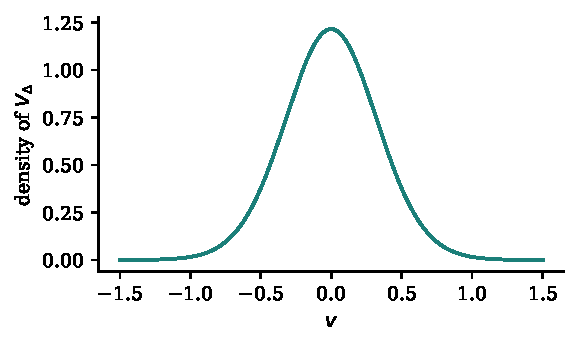
\includegraphics[width=0.75\textwidth]{figs/vdp_delta.pdf}
\caption{The density of $V_\Delta$, the inverse Fourier transform of $t\mapsto\Lambda(6,\Delta)/\Lambda(6+t,\Delta)$, computed from $L$ values for $|t|\le60$ only. It is positive, of mass $0.99995$, with value $1.21546$ at the origin, and log concave on the computed range.}\label{fig:10dvdp}
\end{figure}

For $\Delta$ the partner can be computed without knowing a single zero. We evaluated $g(t) = \Lambda(6,\Delta)/\Lambda(6+t,\Delta)$ on $0\le t\le60$ with PARI/GP and inverted the Fourier transform by quadrature. The result (Figure~\ref{fig:10dvdp}) is a positive density (minimum $2.4\cdot10^{-4}$ on $[0,1.5]$) of total mass $0.99995$, with density $1.21546$ at $0$, and log concave on the computed range. Log concavity is the P\'olya frequency property of order two, so the computation is numerical evidence for the two weakest consequences of Theorem~\ref{thm:10dvdp}(b).

\section{A gallery of van Dantzig pairs and Wald couples}

Each example below is a characteristic function $f$ with a partner $1/f(i\cdot)$ and, where available, a Wald couple. We checked every displayed identity numerically to at least nine digits.

\emph{Cosine and sine.} The function $\cos s = \prod_{k\ge1}(1-4s^2/((2k-1)\pi)^2)$ is the characteristic function of $\pm1$, with partner $1/\cosh s$, the characteristic function of $\sum_k2L_k/((2k-1)\pi)$. Similarly $\sin s/s$, the characteristic function of the uniform law on $(-1,1)$, has partner $s/\sinh s$, the characteristic function of $\sum_kL_k/(k\pi)$, and of the density $\frac\pi4\cosh^{-2}(\pi x/2)$. In the notation of Biane, Pitman and Yor \cite{bpy2001}, $\E e^{-\lambda C} = 1/\cosh\sqrt{2\lambda}$ and $\E e^{-\lambda S} = \sqrt{2\lambda}/\sinh\sqrt{2\lambda}$, so $(\pm1,C/2)$ and $(U,S/2)$, with $U$ uniform on $(-1,1)$, are Wald couples; $C$ and $S$ are hitting times of $1$ by the norms of one and three dimensional Brownian motion started at $0$.\index{Biane Pitman Yor variables}

\emph{Bessel functions and the symmetric Beta laws.} For $\nu>-\frac12$ let $X_\nu$ have the symmetric Beta (power semicircle) density $(1-x^2)^{\nu-1/2}/B(\nu+\frac12,\frac12)$ on $(-1,1)$: the arcsine law for $\nu=0$, the uniform law for $\nu=\frac12$, Wigner's semicircle for $\nu=1$, and the sign $\pm1$ as the limit $\nu\downarrow-\frac12$. Then
\begin{equation}\label{eq:10dbeta}
f_\nu(s) = \E e^{isX_\nu} = \Gamma(\nu+1)\Bigl(\frac s2\Bigr)^{-\nu}J_\nu(s) = \prod_{n\ge1}\Bigl(1-\frac{s^2}{j_{\nu,n}^2}\Bigr),
\end{equation}
with $j_{\nu,n}$ the positive zeros of $J_\nu$ (Exercise~\ref{ex:10dbeta}), and the partner $1/f_\nu(is) = \Gamma(\nu+1)^{-1}(s/2)^\nu/I_\nu(s)$ is the characteristic function of $H_\nu = \sum_nL_n/j_{\nu,n}$ \cite{hinds1974,jurek2010,amdeberhan2012,hasebesimonwang2018}. The case $\nu=\frac12$ is the sine pair above and $\nu=-\frac12$ the cosine pair. The Wald couple is $(X_\nu,T_\nu/2)$ with $T_\nu$ the hitting time of $1$ by a Bessel process of dimension $2\nu+2$ from $0$, whose Laplace transform $(\sqrt{2\lambda}/2)^\nu/(\Gamma(\nu+1)I_\nu(\sqrt{2\lambda}))$ is Kent's \cite{kent1978}.

\emph{Macdonald functions.} P\'olya \cite{polya1926} proved that for $a>0$ the function $t\mapsto K_{it}(a) = \int_0^\infty e^{-a\cosh u}\cos(tu)\,du$ has only real zeros. It is the Fourier transform of the positive even density proportional to $e^{-a\cosh u}$, so $t\mapsto K_{it}(a)/K_0(a)$ lies in $\mathcal D_L$ and $t\mapsto K_0(a)/K_t(a)$ is a characteristic function. Biane \cite{biane2009} gave a probabilistic account of P\'olya's theorem through matrix valued Brownian motion. The kernel $e^{-a\cosh u}$ is the simplest model of the P\'olya kernel of $\xi$, which behaves like $\exp(-\pi e^{2|u|})$.

\emph{Symmetric $z$ laws.} For $\delta>0$ let $G,G'$ be independent with the gamma law of shape $\delta$. Then $X = \log(G/G')$ has
\[
\E e^{isX} = \frac{|\Gamma(\delta+is)|^2}{\Gamma(\delta)^2} = \prod_{k\ge0}\Bigl(1+\frac{s^2}{(\delta+k)^2}\Bigr)^{-1},
\]
and for $\delta>\frac12$ its van Dantzig partner $\Gamma(\delta)^2/(\Gamma(\delta+t)\Gamma(\delta-t)) = \prod_{k\ge0}(1-t^2/(\delta+k)^2)$ is the characteristic function of $2\Theta$, where $\Theta$ has density proportional to $\cos^{2\delta-2}\theta$ on $(-\frac\pi2,\frac\pi2)$, by Cauchy's beta integral (we checked this at $\delta = 1.3$). So $X = \sqrt Y\,N$ is a normal variance mixture with mixing law $Y = \sum_{k\ge0}E_k/\lambda_k$, $\lambda_k = \frac12(\delta+k)^2$, a GGC with Thorin measure $\sum\delta_{\lambda_k}$. Partial fractions give the mixing density as an alternating series,
\[
p_Y(u) = \sum_{k\ge0}\binom{-2\delta}{k}\frac{\delta+k}{B(\delta,\delta)}\,e^{-(\delta+k)^2u/2},\qquad u>0,
\]
whose coefficients alternate in sign although $p_Y\ge0$. For $\delta=0.7$ we checked $\prod_k(1+s/\lambda_k)^{-1} = |\Gamma(\delta+i\sqrt{2s})|^2/\Gamma(\delta)^2$ to all printed digits at $s = 0.1$, $1$, $5$ (values $0.6076958543678661$, $0.04998906407585931$, $2.860474564093928\cdot10^{-4}$), and the Laplace transform of the series above against the product at $s=1.3$ to fifteen digits.

\emph{Gumbel and Hinds.} If $X = -\log E$, the Gumbel law with distribution function $\exp(-e^{-x})$, then
\[
\E e^{-sX} = \Gamma(1+s) = \exp\Bigl(-\gamma_{\mathrm E}s+\int_0^\infty(e^{-st}-1+st)\frac{dt}{t(e^t-1)}\Bigr),\qquad s>-1,
\]
with $\gamma_{\mathrm E}$ Euler's constant. The L\'evy density is $k(t)/t$ with $k(t) = 1/(e^t-1)$ completely monotone, so $X$ is an extended GGC in Bondesson's sense \cite{bondesson1992}. Hinds \cite{hinds1974} considered $X_1$ with density $\frac2{\sqrt\pi}\exp(x-e^{2x})$, that is $X_1 = \frac12\log G$ with $G$ of gamma law of shape $\frac12$, and $X_2 = -X_1$. Their characteristic functions are
\[
f_1(s) = \frac1{\sqrt\pi}\Gamma\Bigl(\frac{1+is}2\Bigr),\qquad f_2(s) = \frac1{\sqrt\pi}\Gamma\Bigl(\frac{1-is}2\Bigr),
\]
with normalisation $1/\sqrt\pi$, as $f_1(0)=1$ requires. Neither lies in $\mathcal D$: $Vf_1(t) = \sqrt\pi/\Gamma(\frac{1-t}2)$ is real but not even, while a real characteristic function is even. Their product, the characteristic function of $X_1-X_1'$ with $X_1'$ an independent copy of $X_1$, is $|\Gamma(\frac{1+is}2)|^2/\pi = 1/\cosh(\pi s/2)$ by the reflection formula, and $V(1/\cosh(\pi\cdot/2))(t) = \cos(\pi t/2)$: the cosine pair again.\index{Hinds pair}

\emph{The reciprocal Gamma function and a Gamma Wald couple.} Hartman \cite{hartman1976} proved that for real $c$ the function $e^{c\sqrt s}/\Gamma(1+\sqrt s)$ is the Laplace transform of a positive infinitely divisible law if and only if $c\le-\gamma_{\mathrm E}$ (see also \cite{roynetteyor2005}). Applying the sine squared lemma of the next section (Lemma~\ref{lem:10dsin2}) to $f=\Gamma$ at $\alpha=1$, whose L\'evy representation is the Gumbel formula above, gives the extreme case $c=-\gamma_{\mathrm E}$ with an explicit Thorin density (this book):
\begin{equation}\label{eq:10dnewman}
\frac{e^{-\gamma_{\mathrm E}\sqrt s}}{\Gamma(1+\sqrt s)} = \E e^{-sH_\Gamma},\qquad u_\Gamma(z) = \frac{\operatorname{Re}\psi(1+i\sqrt z)+\gamma_{\mathrm E}}{2\pi\sqrt z}\ge0,
\end{equation}
with $H_\Gamma$ a GGC of Thorin density $u_\Gamma$, where $\psi = \Gamma'/\Gamma$; positivity is the identity $\operatorname{Re}\psi(1+iy)+\gamma_{\mathrm E} = \sum_{k\ge1}y^2/(k(k^2+y^2))$. We checked \eqref{eq:10dnewman} at $s=2$ to nine digits. The GGC property is stated for the family $\Gamma(\alpha)e^{\sqrt s\,\psi(\alpha)}/\Gamma(\alpha+\sqrt s)$ in \cite{polson2018vdp}, Section~4; the density $u_\Gamma$ is computed here. Since $\E e^{s(\log E+\gamma_{\mathrm E})} = e^{\gamma_{\mathrm E}s}\Gamma(1+s)$, the pair $(\log E+\gamma_{\mathrm E},H_\Gamma)$ is a Wald couple with both members infinitely divisible: in our normalisation it is the couple that Roynette and Yor \cite{roynetteyor2005} build on Hartman's theorem.

\emph{Ostrovskii's hyperbolic class.} Ostrovskii \cite{ostrovskii1970} studied characteristic functions built from hyperbolic functions. In the form presented in the 2018 to 2021 versions of \cite{polson2018vdp}, one takes $f_\delta(z) = z^{-2}-(Cz)^{-1}+\delta\sum_ka_k/(z+h_k)$ with $\frac\pi2<C<B$, $h_k\ge B$, $a_k\ge0$, $\sum a_k<\infty$; then for $\delta$ small $\phi_\delta(t) = f_\delta(\cosh t)/f_\delta(1)$ and $1/\phi_\delta(it) = f_\delta(1)/f_\delta(\cos t)$ are both characteristic functions. The positivity of the Fourier transform of $\phi_\delta$ rests on the elementary integrals
\begin{align*}
\int_{\R}\frac{e^{itx}\,dt}{\cosh t+b} &= \frac{2\pi\sinh((\pi-a)x)}{\sin a\,\sinh\pi x}, & |b|<1,\ \cos a &= -b,\\
\int_{\R}\frac{e^{itx}\,dt}{\cosh t+b} &= \frac{2\pi\sin(ax)}{\sinh a\,\sinh\pi x}, & b>1,\ \cosh a &= b,
\end{align*}
and $\int e^{itx}\cosh^{-2}t\,dt = \pi x/\sinh(\pi x/2)$, which we verified (those versions misprint the second condition as $\cosh a = -b$). We refer to \cite{ostrovskii1970} for the precise class and do not reproduce the estimates.

\section{The sine squared transport}\index{sine squared transport}

The Thorin densities of this book have so far been read off from zeros. The following lemma, the $2\sin^2$ lemma of \cite{polson2018vdp} (Lemma~14 there; see also \cite{polson2017}, Section~5), produces them from the L\'evy measure of $\log f$ at a basepoint, which for an $L$ function is the arithmetic. Its first step, which writes $e^{-x\sqrt s}-1+x\sqrt s$ through the positive $\frac12$ stable law, is Th\'eor\`eme~I.1.1 of Roynette and Yor \cite{roynetteyor2005}, which also shows that the resulting $H$ is self decomposable. We state the lemma in our normalisation and prove it.

\begin{lemma}[sine squared lemma]\label{lem:10dsin2}
Let $f$ be holomorphic and zero free on $\operatorname{Re}w>\alpha-\eta$ for some $\eta>0$, positive on $(\alpha,\infty)$, and suppose that for $s\ge0$
\begin{equation}\label{eq:10dlk}
\log f(\alpha+s)-\log f(\alpha)-bs = \int_0^\infty(e^{-sx}-1+sx)\,\frac{\nu(dx)}x,\qquad b = \frac{f'(\alpha)}{f(\alpha)},
\end{equation}
with $\nu$ a positive measure on $(0,\infty)$ such that $\int_0^\infty\min(1,x)\,\nu(dx)<\infty$. Then for $s>0$
\[
\frac{f(\alpha)}{f(\alpha+\sqrt s)} = e^{-b\sqrt s}\,\E e^{-sH},
\]
where $H$ is a GGC with drift zero and Thorin density
\begin{equation}\label{eq:10dU}
U(z) = \frac1{2\pi\sqrt z}\int_0^\infty2\sin^2\Bigl(\frac{x\sqrt z}2\Bigr)\nu(dx) = \frac{\operatorname{Re}(f'/f)(\alpha+i\sqrt z)-b}{2\pi\sqrt z}.
\end{equation}
If $b\ge0$, $e^{-b\sqrt s}$ is the Laplace transform of a positive $\frac12$ stable law, a GGC with Thorin density $b/(2\pi\sqrt z)$, and then $f(\alpha)/f(\alpha+\sqrt s)$ is itself a GGC transform with Thorin density $\operatorname{Re}(f'/f)(\alpha+i\sqrt z)/(2\pi\sqrt z)$. The hypothesis \eqref{eq:10dlk} with $\nu\ge0$ holds if and only if $s\mapsto(\log f)''(\alpha+s)$ is completely monotone on $(0,\infty)$ and tends to $0$ at infinity.
\end{lemma}

\begin{proof}
\emph{Step 1: subordination.} For $x>0$ the positive $\frac12$ stable density $q_x(y) = \frac x{2\sqrt\pi}y^{-3/2}e^{-x^2/(4y)}$ has $\int_0^\infty e^{-sy}q_x(y)\,dy = e^{-x\sqrt s}$, and $\int_0^\infty(1-e^{-sy})y^{-3/2}dy = 2\sqrt\pi\sqrt s$ (substitute $u = sy$ and integrate by parts). Hence
\begin{align*}
e^{-x\sqrt s}-1+x\sqrt s &= \int_0^\infty(1-e^{-sy})\Bigl[\frac x{2\sqrt\pi}y^{-3/2}-q_x(y)\Bigr]dy\\
&= \int_0^\infty(1-e^{-sy})K(x,y)\,dy,
\end{align*}
with $K(x,y) = \frac x{2\sqrt\pi\,y^{3/2}}(1-e^{-x^2/(4y)})\ge0$.

\emph{Step 2: a Laplace pair.} For $a\ge0$ and $y>0$,
\begin{equation}\label{eq:10dpair}
\frac{1-e^{-a/y}}{\sqrt y} = \int_0^\infty e^{-yz}\,\frac{2\sin^2\sqrt{az}}{\sqrt{\pi z}}\,dz .
\end{equation}
Indeed $\int_0^\infty e^{-yz}(\pi z)^{-1/2}dz = y^{-1/2}$, and expanding the cosine,
\[
\int_0^\infty\frac{e^{-yz}\cos(2\sqrt{az})}{\sqrt{\pi z}}\,dz = \sum_{n\ge0}(-1)^n\frac{4^na^n\,\Gamma(n+\frac12)}{(2n)!\sqrt\pi\,y^{n+1/2}} = \frac{e^{-a/y}}{\sqrt y},
\]
using $\Gamma(n+\frac12) = (2n)!\sqrt\pi/(4^nn!)$; the interchange is justified by the bound $\cosh(2\sqrt{az})$ for the absolute series, which is integrable against $e^{-yz}z^{-1/2}$. Subtract and use $1-\cos2\theta = 2\sin^2\theta$.

\emph{Step 3: the L\'evy density.} Replace $s$ by $\sqrt s$ in \eqref{eq:10dlk} and insert Step 1. All integrands are nonnegative, so Tonelli's theorem gives
\[
\log\frac{f(\alpha+\sqrt s)}{f(\alpha)}-b\sqrt s = \int_0^\infty(1-e^{-sy})\frac{k(y)}y\,dy,
\]
with $k(y) = (4\pi y)^{-1/2}\int_0^\infty(1-e^{-x^2/(4y)})\,\nu(dx)$. By \eqref{eq:10dpair} with $a = x^2/4$ and Tonelli again, $k(y) = \int_0^\infty e^{-yz}U(z)\,dz$ with $U$ the first expression in \eqref{eq:10dU}. Frullani's integral $\int_0^\infty(1-e^{-sy})e^{-zy}y^{-1}dy = \log(1+s/z)$ then gives $\log(f(\alpha+\sqrt s)/f(\alpha))-b\sqrt s = \int_0^\infty\log(1+s/z)U(z)\,dz$, finite for each $s>0$. Finiteness for $s=1$ forces $\int_0^1|\log z|U(z)dz<\infty$ and $\int_1^\infty U(z)z^{-1}dz<\infty$, the integrability conditions of Definition~\ref{def:ch10ggc}, so $\exp(-\int\log(1+s/z)U(z)dz)$ is the transform of a GGC $H$.

\emph{Step 4: the closed form.} Differentiating \eqref{eq:10dlk}, $(f'/f)(\alpha+s)-b = \int_0^\infty(1-e^{-sx})\nu(dx)$ for $s>0$. The right side converges absolutely and uniformly for $\operatorname{Re}s\ge0$ because $|1-e^{-sx}|\le\min(2,|s|x)$, so it is continuous there and holomorphic inside; the left side is holomorphic on $\operatorname{Re}s>-\eta$. They agree for $\operatorname{Re}s\ge0$, and at $s = ir$ the real part of the right side is $\int(1-\cos rx)\nu(dx) = \int2\sin^2(rx/2)\nu(dx)$, which gives the second expression in \eqref{eq:10dU}.

\emph{Step 5.} $\int_0^\infty\log(1+s/z)z^{-1/2}dz = 2\pi\sqrt s$ (substitute $z = su$), so $b\sqrt s = \int\log(1+s/z)\,b(2\pi\sqrt z)^{-1}dz$, which is the stated GGC form of $e^{-b\sqrt s}$. Finally, \eqref{eq:10dlk} gives $(\log f)''(\alpha+s) = \int_0^\infty xe^{-sx}\nu(dx)$, completely monotone and tending to $0$. Conversely Bernstein's theorem writes such a function as $\int_{(0,\infty)}e^{-sx}m(dx)$ with $m\ge0$ and no atom at $0$; integrating twice from $0$ gives \eqref{eq:10dlk} with $\nu(dx) = m(dx)/x$.
\end{proof}

The second form of \eqref{eq:10dU} is Stieltjes inversion in disguise: on the cut $s = -z$ the principal root is $\sqrt s = i\sqrt z$. It shows that \emph{the transported Thorin density can be computed from $f$ alone on one vertical line}. The hypothesis $\nu\ge0$ is sufficient, not necessary, and fails for completed $L$ functions. The next theorem replaces it by a Hadamard argument.

\begin{theorem}[Shifted Thorin representation; this book, extending \cite{polson2017,polson2018vdp}]\label{thm:10dshift}
Let $\pi$ be as in Theorem~\ref{thm:10bmain}, or $\zeta$, and $a>0$. Put
\[
V_a(z) = \frac{\operatorname{Re}(\Xi_\pi'/\Xi_\pi)(a+i\sqrt z)}{2\pi\sqrt z},\qquad z>0 .
\]
\begin{enumerate}
\item[(i)] If every zero $z_k$ of $\Xi_\pi$ satisfies $|\operatorname{Re}z_k|<a$, then $V_a\ge0$ and $\Xi_\pi(a)/\Xi_\pi(a+\sqrt s) = \E e^{-sH_a}$ for $s>0$, with $H_a$ a GGC of drift zero and Thorin density $V_a$.
\item[(ii)] If $\Xi_\pi(a)/\Xi_\pi(a+\sqrt s)$ is a GGC transform on $(0,\infty)$, every zero satisfies $|\operatorname{Re}z_k|\le a$.
\item[(iii)] Unconditionally, (i) holds for every $a\ge\frac12$, that is for every basepoint $\alpha = \frac12+a\ge1$ in the variable $s$ of $\Lambda(s,\pi)$ in the unitary normalisation.
\item[(iv)] GRH for $\pi$ holds if and only if $V_a\ge0$ for every $a>0$, if and only if the conclusion of (i) holds for every $a>0$. Under GRH, $V_a(z)\,dz\to\sum_k\delta_{\gamma_k^2}$ vaguely and $H_a\to Z_\pi$ in law as $a\downarrow0$.
\end{enumerate}
\end{theorem}

\begin{proof}
(i) For $c\in\C$ with $\operatorname{Re}c>0$ and $s>0$, closing the contour in the lower half plane, where the only pole is $r = -i\sqrt s$,
\[
\frac1{2\pi}\int_{-\infty}^\infty\frac{dr}{(c+ir)(s+r^2)} = \frac1{2\sqrt s\,(c+\sqrt s)} .
\]
Taking real parts, and adding the same identity for $\bar c$, the integrand $\operatorname{Re}\frac1{c+ir}+\operatorname{Re}\frac1{\bar c+ir}$ is even in $r$ and positive, and the substitution $z = r^2$ gives
\[
\frac d{ds}\log\Bigl|1+\frac{\sqrt s}c\Bigr|^2 = \int_0^\infty\frac{v_c(z)\,dz}{s+z},
\]
with $v_c(z) = [\operatorname{Re}(c+i\sqrt z)^{-1}+\operatorname{Re}(\bar c+i\sqrt z)^{-1}]/(2\pi\sqrt z)>0$; for real $c>0$ use $c$ alone and halve. Integrating from $0$ (Tonelli) gives $\log|1+\sqrt s/c|^2 = \int_0^\infty\log(1+s/z)v_c(z)\,dz$. Now $\Xi_\pi(w) = \Xi_\pi(0)\prod_k(1-w^2/z_k^2)$, so
\[
\frac{\Xi_\pi(a+w)}{\Xi_\pi(a)} = \prod_k\Bigl(1+\frac w{a-z_k}\Bigr)\Bigl(1+\frac w{a+z_k}\Bigr),
\]
the product over pairs converging absolutely because each pair factor is $1+O((|w|+|w|^2)|z_k|^{-2})$. The numbers $c = a\mp z_k$ have positive real part by hypothesis and form a set closed under conjugation. Summing the single factor identities over this set (Tonelli), and halving because $c$ and $\bar c$ both occur, gives $\log(\Xi_\pi(a+\sqrt s)/\Xi_\pi(a)) = \int\log(1+s/z)V_a(z)\,dz$, because $\sum_c\operatorname{Re}(c+i\sqrt z)^{-1} = \operatorname{Re}\sum_k[(a+i\sqrt z-z_k)^{-1}+(a+i\sqrt z+z_k)^{-1}] = \operatorname{Re}(\Xi_\pi'/\Xi_\pi)(a+i\sqrt z)$. The integrability conditions follow as in Step 3 of Lemma~\ref{lem:10dsin2}.

(ii) By Lemma~\ref{lem:ch10nonvanish} the GGC transform $\varphi$ is holomorphic and zero free on $\C\setminus(-\infty,0]$, and $s\mapsto\Xi_\pi(a+\sqrt s)$ is holomorphic there; the identity $\varphi(s)\Xi_\pi(a+\sqrt s) = \Xi_\pi(a)$ on $(0,\infty)$ extends, so $\Xi_\pi(a+w)\ne0$ for $\operatorname{Re}w>0$. By evenness there is no zero with $\operatorname{Re}z<-a$.

(iii) By Lemma~\ref{lem:10bcompletion}(iii) all zeros satisfy $|\operatorname{Re}z_k|<\frac12$.

(iv) Under GRH, $\operatorname{Re}z_k = 0<a$ for all $k$, so (i) applies for every $a>0$. Conversely suppose $V_a\ge0$ for all $a>0$, and let $z_0$ be a zero of multiplicity $m$ with $\beta = \operatorname{Re}z_0>0$. For small $\eta\in(0,\beta)$, $(\Xi_\pi'/\Xi_\pi)(z_0-\eta) = -m/\eta+O(1)$, whose real part is negative; but $z_0-\eta = a+iy$ with $a = \beta-\eta>0$, and $V_a(y^2)\ge0$ says $\operatorname{Re}(\Xi'_\pi/\Xi_\pi)(a+iy)\ge0$ (for $y\ne0$; if $y=0$, then $z_0$ is real and the same argument applies to $(\Xi_\pi'/\Xi_\pi)(a)$, which is the limit of $\operatorname{Re}(\Xi'_\pi/\Xi_\pi)(a+iy)$ as $y\to0$). This contradiction and evenness give GRH; the second equivalence follows from (i) and (ii). For the limit, under GRH $\operatorname{Re}(\Xi_\pi'/\Xi_\pi)(a+ir) = \sum_{\gamma_k>0}[P_a(r-\gamma_k)+P_a(r+\gamma_k)]$ with the Poisson kernel $P_a(u) = a/(a^2+u^2)$, and $\frac1{2\pi r}P_a(r-\gamma)\,2r\,dr\to\delta_\gamma$ in the variable $r$, that is $\delta_{\gamma^2}$ in $z$; the terms $P_a(r+\gamma_k)$ tend to zero, uniformly summable. Convergence of the transforms, $\Xi_\pi(a)/\Xi_\pi(a+\sqrt s)\to\Xi_\pi(0)/\Xi_\pi(\sqrt s)$, gives convergence in law.
\end{proof}

For $\xi$, parts (i) to (iii) and the limit in (iv) are Theorem~18 and Remark~21 of \cite{polson2018vdp}, and \cite{polson2017} relates the family $\xi(\alpha)/\xi(\alpha+\sqrt s)$ to the criterion of Hinkkanen \cite{hinkkanen1997} and Lagarias \cite{lagarias1999}: the Riemann hypothesis holds if and only if $\operatorname{Re}\xi'/\xi(s)>0$ for $\operatorname{Re}s>\frac12$. Part (iv) is a Thorin form of that criterion. Parts (i) and (ii) are the parabolic picture of Section~\ref{sec:10bparabola} seen from a shifted basepoint: the Thorin property at $a$ is sandwiched between the conditions $\Theta_\sigma$ with $\sigma<a$ and $\sigma = a$. A zero $z_0 = \beta+i\gamma$ of $\Xi_\pi$ with $\beta>a$ would contribute \emph{locally} a negative dip to $V_a$ near $z = \gamma^2$, of depth about $(\beta-a)^{-1}/(2\pi\gamma)$. Chapter~\ref{ch:squarefree} splits these densities for $\xi$ into the contributions of single pairs of zeros, with a Brownian subordination (Corollary~\ref{cor:sf:sub}), Chapter~\ref{ch:beta} studies $V_a$ for $L(s,\chi_{-4})$, and Chapter~\ref{ch:scholze} computes the Thorin measure itself, as a signed density smoothed at width $\varepsilon$, by Stieltjes inversion. For self dual $\pi$, Chapter~\ref{ch:lap} writes $V_a$, halved by passing to $\Xi^{\mathrm{sd}}_\pi$, in the variable $r=\sqrt z$, as a superposition over the zeros of folded Cauchy laws of scales $a-\beta$, so that moving the basepoint adds Cauchy noise (Theorem~\ref{thm:lapcauchy}).

\subsection{At the centre: from the cosine measure to the zeros}

Formally, for real $\gamma>0$ and $\operatorname{Re}z>0$, Frullani's integral with an Abel damping gives
\begin{align*}
\log\Bigl(1+\frac{z^2}{\gamma^2}\Bigr) &= \lim_{\epsilon\downarrow0}2\int_0^\infty\bigl(e^{-\epsilon x}-e^{-(z+\epsilon)x}\bigr)\cos(\gamma x)\frac{dx}x\\
&= \int_0^\infty(1-e^{-zx})\,2\cos(\gamma x)\frac{dx}x,
\end{align*}
so that under GRH, $\log(\Xi_\pi(z)/\Xi_\pi(0)) = -\int_0^\infty(e^{-zx}-1+zx)\mu(dx)/x$ formally, with the \emph{cosine L\'evy measure}\index{cosine L\'evy measure} $\mu(dx) = 2\sum_k\cos(\gamma_kx)\,dx$ (the linear term vanishes because $\Xi_\pi'(0) = 0$). Insert $-\mu$ for $\nu$ in the first form of \eqref{eq:10dU} at $\alpha = 0$. As distributions in $r = \sqrt z>0$, we have $\int_0^\infty\cos(\gamma x)dx = 0$ and $\int_0^\infty\cos(rx)\cos(\gamma x)dx = \frac\pi2\delta(r-\gamma)$, so
\begin{align*}
U(z) &= -\frac1{2\pi r}\sum_k2\int_0^\infty(1-\cos rx)\cos(\gamma_kx)\,dx\\
&= \frac1{2r}\sum_k\delta(r-\gamma_k) = \sum_k\delta(z-\gamma_k^2),
\end{align*}
using $\delta(\sqrt z-\gamma) = 2\gamma\,\delta(z-\gamma^2)$. \emph{The sine squared transport carries the cosine measure of the zeros exactly to the Thorin measure $\sum_k\delta_{\gamma_k^2}$.} The damping $e^{-\epsilon x}$ makes this rigorous: it is the shift $a = \epsilon$, and the computation becomes Theorem~\ref{thm:10dshift}.

\begin{proposition}[this book]\label{prop:10dsmooth}
Assume GRH for $\pi$ and let $\epsilon>0$. With $P_\epsilon(u) = \epsilon/(\epsilon^2+u^2)$ and $b_\epsilon = (\Xi_\pi'/\Xi_\pi)(\epsilon) = \sum_{\gamma_k>0}2P_\epsilon(\gamma_k)$,
\begin{gather*}
\frac{\Xi_\pi(\epsilon)}{\Xi_\pi(\epsilon+\sqrt s)} = e^{-b_\epsilon\sqrt s}\exp\Bigl(-\int_0^\infty\log\Bigl(1+\frac sz\Bigr)U_\epsilon(z)\,dz\Bigr),\\
U_\epsilon(z) = \frac1{2\pi\sqrt z}\sum_{\gamma_k>0}\bigl[P_\epsilon(\sqrt z-\gamma_k)+P_\epsilon(\sqrt z+\gamma_k)-2P_\epsilon(\gamma_k)\bigr],
\end{gather*}
and $U_\epsilon(z) = (2\pi\sqrt z)^{-1}\int_0^\infty2\sin^2(x\sqrt z/2)e^{-\epsilon x}(-\mu)(dx)$ is the sine squared transport of the damped cosine measure.
\end{proposition}

\begin{proof}
$U_\epsilon = V_\epsilon-b_\epsilon/(2\pi\sqrt z)$ in the notation of Theorem~\ref{thm:10dshift}, and the identity is (i) of that theorem combined with Step 5 of Lemma~\ref{lem:10dsin2}. The transport formula is the elementary integral $\int_0^\infty(1-\cos rx)\cos(\gamma x)e^{-\epsilon x}dx = P_\epsilon(\gamma)-\frac12[P_\epsilon(r-\gamma)+P_\epsilon(r+\gamma)]$, summed over $k$.
\end{proof}

\begin{figure}[t]
\centering
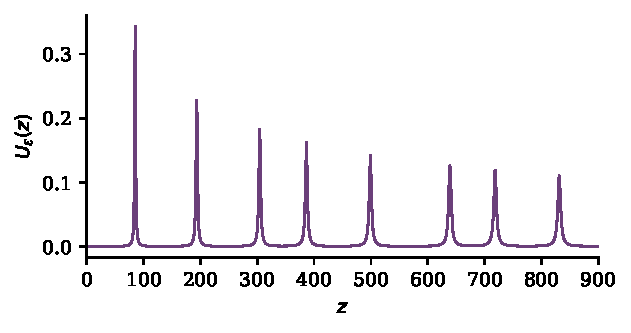
\includegraphics[width=0.78\textwidth]{figs/sin2_transport.pdf}
\caption{The sine squared transport $U_\epsilon(z)$ of the damped cosine L\'evy measure $2\sum_k\cos(\gamma_kx)e^{-0.05x}$ over the first $60$ zeros of $\Delta$: a smoothed Thorin density with peaks at $\gamma_k^2$, mass $0.983$ within $30$ of $\gamma_1^2 = 85.052$.}\label{fig:10dsin2}
\end{figure}

For $\Delta$, with $\epsilon = 0.05$ and the first $60$ zeros, $U_\epsilon$ is positive on $4\le z\le900$ (minimum $2.0\cdot10^{-5}$) with peaks at the $\gamma_k^2$ and mass $0.983$ within $30$ of $\gamma_1^2 = 85.052$, unit mass up to the smoothing loss (Figure~\ref{fig:10dsin2}). Since $U_\epsilon$ contains the negative term $-b_\epsilon/(2\pi\sqrt z)$, its positivity is a property of the zeros and not of the construction.

\subsection{The explicit formula: from the primes to the Thorin measure}\index{explicit formula}

The cosine measure is the Fourier transform of the zero counting measure, and Weil's explicit formula (Theorem~\ref{thm:10cexplicit} for $\Delta$; \cite{weil1952,iwanieckowalski2004} in general) computes that transform. Let $\pi$ be self dual with $\Lambda(\frac12,\pi)\ne0$, and write $-L'/L(s,\pi) = \sum_n\Lambda_\pi(n)n^{-s}$ in the unitary normalisation. Taking for $h$ the cosine kernel, the formula reads, as an identity of distributions on $(0,\infty)$,
\begin{equation}\label{eq:10dweil}
\mu(dx) = 2\sum_{\gamma_k>0}\cos(\gamma_kx)\,dx = -\sum_{n\ge2}\frac{\Lambda_\pi(n)}{\sqrt n}\,\delta_{\log n}(dx)+A_\pi(x)\,dx,
\end{equation}
where $A_\pi$ is the archimedean density, the Fourier transform of $\frac1{2\pi}2\operatorname{Re}[\frac{\gamma'}{\gamma}(\frac12+it,\pi)]$; for $\zeta$ the right side also contains the polar term $2\cosh(x/2)\,dx$. Combining \eqref{eq:10dweil} formally with the transport: \emph{the Thorin density of $1/F_\pi$ is the sine squared transform of the explicit formula distribution, and GRH is its positivity.} Since the transport acts on $\nu = -\mu$, the atom at $\log n$ contributes $+\Lambda_\pi(n)n^{-1/2}(2\pi\sqrt z)^{-1}2\sin^2(\frac12\sqrt z\log n)$, of the sign of $\Lambda_\pi(n)$, and for $\Delta$ the atoms of \eqref{eq:10dweil} at $\log p^m$, $m\ge1$, are, up to sign and the factor $p^{-m/2}$, the corresponding atoms of the Fourier transform of the local Thorin comb of $p$ (Proposition~\ref{prop:10cdictionary}); only the sum over all $n$ together with $A_\pi$ is concentrated on the $\gamma_k^2$.\index{heat trace}

The rigorous form of this statement uses test functions. The heat trace
\[
\mathcal W_\pi(x) = k_\pi(x) = \sum_ke^{-x\gamma_k^2},
\]
summed over the pairs $\pm z_k = \pm i\gamma_k$ of \eqref{eq:10batoms}, formed from $\Xi^{\mathrm{sd}}_\pi$ when $\pi$ is self dual, so that each zero of $\Lambda(s,\pi)$ counts once, as in Table~\ref{tab:10dheat}, is the L\'evy function of Theorem~\ref{thm:10bmain}(d), so \emph{GRH holds if and only if $\mathcal W_\pi$ is completely monotone}. For $\xi$ the first author states in \cite{polson2018vdp} (Theorems~22 and~26) that the heat trace is positive and strictly decreasing unconditionally, so that the law with Laplace transform $\xi(\frac12)/\xi(\frac12+\sqrt s)$ is self decomposable, and that its complete monotonicity is equivalent to the Riemann hypothesis; the second statement is the case $\pi = \zeta$ of Theorem~\ref{thm:10bmain}, and we do not use the first. With $h(t) = t^{2n}e^{-xt^2}$ in Weil's formula, $(-1)^n\mathcal W^{(n)}(x) = \sum\gamma_k^{2n}e^{-x\gamma_k^2}$ is a sum over primes plus an archimedean integral. Since the transform $H(y)$ of $h$ in Theorem~\ref{thm:10cexplicit} then decays like $e^{-y^2/(4x)}$, only primes with $\log p\le\sqrt{240x}+1$ matter at double precision: $p\le24$ at $x = 0.02$ and $p\le365$ at $x = 0.1$. For $\Delta$ we obtained, from the zeros and independently from the primes, the values in Table~\ref{tab:10dheat}: agreement to thirteen to sixteen significant digits, with the complete monotonicity signs through $n=3$. Small $x$ needs only a few primes and is dominated by the archimedean term; large $x$ and high derivative orders need many primes, and that is where individual ordinates are resolved.

\begin{table}[t]
\centering\footnotesize
\begin{tabular}{llll}
\toprule
$x$ & quantity & from the zeros & from the primes\\
\midrule
$0.02$ & $\mathcal W$ & $0.2061515276408161$ & $0.20615152764081612$\\
 & $-\mathcal W'$ & $20.450633094275233$ & $20.450633094275236$\\
 & $\mathcal W''$ & $2391.2851645202795$ & $2391.2851645202795$\\
 & $-\mathcal W'''$ & $359738.32402760646$ & $359738.3240276065$\\
$0.05$ & $\mathcal W$ & $0.014290332953786858$ & $0.01429033295378686$\\
 & $-\mathcal W'''$ & $9216.990197017574$ & $9216.99019701757$\\
$0.1$ & $\mathcal W$ & $2.0241135580126968\cdot10^{-4}$ & $2.0241135580125608\cdot10^{-4}$\\
 & $-\mathcal W'''$ & $124.56174145637718$ & $124.56174145637709$\\
\bottomrule
\end{tabular}
\caption{The heat trace $\mathcal W(x) = \sum_{\gamma>0}e^{-x\gamma^2}$ of $\Delta$ and its derivatives, from the zeros and from the primes through Weil's explicit formula.}\label{tab:10dheat}
\end{table}

Figure~\ref{fig:10dheatfig} plots the same quantities as functions of $x$.

\begin{figure}[ht]\centering
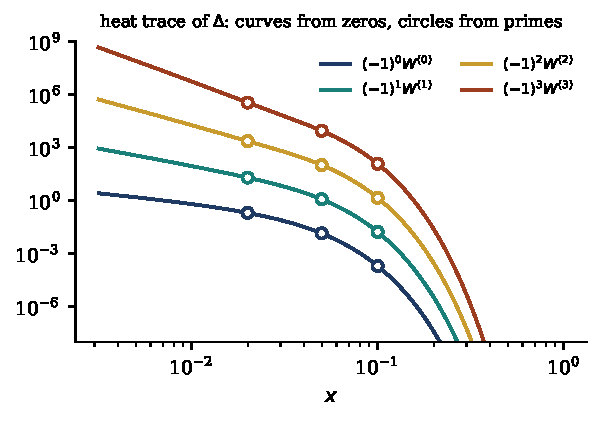
\includegraphics[width=0.9\textwidth]{figs/heattrace_primes.pdf}
\caption{Heat trace $\mathcal W$ of $\Delta$ and its first three derivatives with alternating signs. Curves: sums over the zeros up to height 300. Circles: Weil's explicit formula, using only the primes and the archimedean term. Complete monotonicity is the statement that every such curve is positive for every $n$.}\label{fig:10dheatfig}
\end{figure}

\begin{figure}[t]
\centering
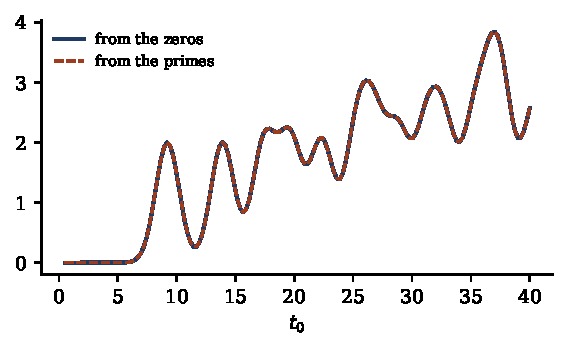
\includegraphics[width=0.78\textwidth]{figs/zeros_from_primes.pdf}
\caption{Zeros from primes for $\Delta$: the smoothed zero count $\sum_{\gamma}[e^{-(\gamma-t_0)^2/2}+e^{-(\gamma+t_0)^2/2}]$ from the zeros and from the primes $p\le1.6\cdot10^5$ with the archimedean term. Maximal difference $4.0\cdot10^{-14}$ for $t_0\in[0.5,40]$.}\label{fig:10dprimes}
\end{figure}

The same mechanism recovers the zeros themselves: in Figure~\ref{fig:10dprimes} the smoothed zero count of $\Delta$ computed from the primes agrees with that computed from the zeros to $4.0\cdot10^{-14}$, against a peak value of $3.84$.

\subsection{Away from the centre}\label{sec:10daway}

For $\alpha>1$ the Euler product gives the L\'evy measure of $\log L(\alpha+s,\pi)$ explicitly:
\[
\log\frac{L(\alpha+s,\pi)}{L(\alpha,\pi)}-s\frac{L'}L(\alpha,\pi) = \sum_{n\ge2}\frac{\Lambda_\pi(n)}{n^\alpha\log n}\bigl(e^{-s\log n}-1+s\log n\bigr),
\]
so $\nu_{\mathrm{ar}} = \sum_n\Lambda_\pi(n)n^{-\alpha}\delta_{\log n}$, whose transport is
\[
U_{\mathrm{ar}}(z) = \frac1{2\pi\sqrt z}\sum_{n\ge2}\frac{\Lambda_\pi(n)}{n^\alpha}\,2\sin^2\Bigl(\frac{\sqrt z\log n}2\Bigr).
\]
Chapter~\ref{ch:lap} inverts this transport, signed or not, by Gaussian means and recovers the $\Lambda_\pi(n)$ (Corollary~\ref{cor:lapfrob}). For $\zeta$, for Dedekind zeta functions and for the Rankin Selberg function $L(s,\pi\times\tilde\pi)$, either partial, as $L^S$ with $S$ a finite set of primes containing the ramified ones, or complete (Theorem~\ref{thm:ch09rs} and the paragraph after it), the coefficients $\Lambda_\pi(n)$ are nonnegative, so $U_{\mathrm{ar}}\ge0$. The completed function adds two archimedean pieces of opposite sign. Binet's formula $(\log\Gamma)''(w) = \int_0^\infty te^{-wt}(1-e^{-t})^{-1}dt$ shows that $\log\Gamma((\alpha+s)/2)$ contributes the positive density $e^{-\alpha x}(1-e^{-2x})^{-1}$ to $\nu$, while Frullani's integral shows that the polynomial factors $s(s-1)$ of $\xi$ contribute $-(e^{-\alpha x}+e^{-(\alpha-1)x})$, a negative density. Hence $\nu$ is a signed measure for $\xi$ and Lemma~\ref{lem:10dsin2} does not apply as stated; what must be checked is the positivity of the \emph{total} transported density. The first author discusses this decomposition in \cite{polson2018vdp} (Remark~19) and obtains the Thorin representation of $\xi(\alpha)/\xi(\alpha+\sqrt s)$ for $\alpha\ge1$ from the Hadamard product instead, as Theorem~\ref{thm:10dshift}(iii) does for every $\Xi_\pi$. For signed coefficients, as for $L(s,\chi)$ with $\chi$ real taking the value $-1$, or $L(s,\Delta)$, the arithmetic part $\nu_{\mathrm{ar}}$ is itself signed, and for complex $\chi$ it is complex; one must then work with the completion $\Xi_\chi$ of Chapter~\ref{ch:10b}. Inside the critical strip the question is of Riemann hypothesis type: by the argument of Theorem~\ref{thm:10dshift}(iv), nonnegativity of $V_{a'}$ for every $a'\ge a$ excludes zeros of $\Lambda(s,\pi)$ with real part above $\frac12+a$.

We computed the density $U$ of \eqref{eq:10dU}, in its second form, at the $15000$ points $\sqrt z=0.01,0.02,\dots,150$, for $\xi$ at $\alpha = 0.55, 0.75, 0.99, 1.25, 2$ and for $\Delta$ at the basepoints $6+\alpha-\frac12$ of $\Lambda(s,\Delta)$, the same offsets $\alpha-\frac12$ from the centre; it is positive at every point in every case, with its minimum at $\sqrt z=0.01$, where $U$ vanishes like a multiple of $\sqrt z$ (the value there is $1.8\cdot10^{-8}$ for $\xi$ at $\alpha = 0.55$ and $9.5\cdot10^{-8}$ for $\Delta$ at the same $\alpha$). These are numerical observations at every $\alpha$, and the grid sees only zeros of height below $150$. For $\alpha\ge1$, Theorem~\ref{thm:10dshift}(iii) proves only $V_{\alpha-1/2}\ge0$; since $U = V_{\alpha-1/2}-b/(2\pi\sqrt z)$ with $b>0$, positivity of $U$ is a stronger statement: for $\xi$ it says that $\operatorname{Re}\xi'/\xi$ is smallest on the real axis along the line $\operatorname{Re}s=\alpha$. Lagarias \cite{lagarias1999} proved this under the Riemann hypothesis for every $\alpha>\frac12$, and unconditionally for $\alpha\ge10$; Garunk\v{s}tis lowered the unconditional range to $\alpha>4.5$ \cite{garunkstis2000} and then to $\alpha\ge1$ \cite{garunkstis2002}. Unconditionally it is open only for $\frac12<\alpha<1$, where Chapter~\ref{ch:beta} proves it up to the height to which the Riemann hypothesis is verified, with the analogue for $L(s,\chi_{-4})$ (Theorem~\ref{beta:thm:minall}). Chapter~\ref{ch:recip} builds the corresponding family for the Rankin Selberg square of an Artin representation from its Frobenius traces, keeping the poles of the completed $L$ function, so that no polynomial factor contributes a negative density; there the densities are nonnegative for $\alpha>1$ (Proposition~\ref{prop:recipfamily}), and below $\alpha=1$ the same question is Open Problem~\ref{op:recipdescent}.

\section{Subordinators of L functions and hitting times}\index{zeta subordinator}

Fix $\sigma>1$. Since $\log\zeta(\sigma+\lambda)-\log\zeta(\sigma) = -\sum_{n\ge2}\frac{\Lambda(n)}{n^\sigma\log n}(1-n^{-\lambda})$, the function $\lambda\mapsto\log(\zeta(\sigma)/\zeta(\sigma+\lambda))$ is a Bernstein function with L\'evy measure $\Pi_\sigma = \sum_n\frac{\Lambda(n)}{n^\sigma\log n}\delta_{\log n}$ of total mass $\log\zeta(\sigma)$. Let $X_t$ be the compound Poisson subordinator with this L\'evy measure:
\[
\E e^{-\lambda X_t} = \Bigl(\frac{\zeta(\sigma+\lambda)}{\zeta(\sigma)}\Bigr)^t,\qquad\lambda\ge0,\ t\ge0 .
\]
Let $d_t(m)$ be the Dirichlet coefficients of $\zeta^t$, defined as $\exp(t\log\zeta)$: $d_t$ is multiplicative with $d_t(p^k) = \binom{t+k-1}k$.

\begin{proposition}[this book]\label{prop:10dsublaw}
For $t>0$, $X_t$ takes values in $\{\log m:m\ge1\}$ and $\Prob(X_t = \log m) = d_t(m)m^{-\sigma}/\zeta(\sigma)^t$.
\end{proposition}

\begin{proof}
The jumps of $X$ lie in $\{\log n\}$, so $X_t$ is the logarithm of a product of integers. For $\operatorname{Re}s>1$ the Euler product gives
\[
\zeta(s)^t = \prod_p(1-p^{-s})^{-t} = \prod_p\sum_k\binom{t+k-1}kp^{-ks} = \sum_md_t(m)m^{-s},
\]
with $d_t(m)\ge0$. Hence $\E e^{-\lambda X_t} = \sum_m d_t(m)m^{-\sigma}\zeta(\sigma)^{-t}e^{-\lambda\log m}$ for $\lambda\ge0$, and the coefficients sum to $1$ at $\lambda = 0$. A law on $[0,\infty)$ is determined by its Laplace transform.
\end{proof}

As $\sigma\downarrow1$ the ranked normalised sizes of the prime factors of the integer $e^{X_t}$ converge in law to the Poisson Dirichlet law with parameter $t$ (Theorem~\ref{thm:pdtheta}), so that the zeta subordinator carries the whole Ewens family.

Let $c>0$ and $Z_t = t/c-X_t$, a spectrally negative L\'evy process of bounded variation with drift $1/c$. Its Laplace exponent $\psi(\lambda) = \log\E e^{\lambda Z_1} = \lambda/c+\log(\zeta(\sigma+\lambda)/\zeta(\sigma))$ is convex on $[0,\infty)$ with $\psi(0)=0$ and $\psi(\lambda)\to\infty$; let $\Phi$ be its right inverse. Let $\tau_x = \inf\{t:Z_t>x\}$ for $x>0$. Since $Z$ moves up only continuously, $Z_{\tau_x} = x$ on $\{\tau_x<\infty\}$, so
\[
\tau_x = c\bigl(x+\log M_x\bigr),\qquad M_x = e^{X_{\tau_x}}\in\{1,2,3,\dots\}.
\]
We use two classical facts: $\E e^{-q\tau_x} = e^{-x\Phi(q)}$ for $q\ge0$ \cite{bertoin1996,kyprianou2014}, and Kendall's identity \cite{kendall1957,bertoin1996,kyprianou2014}: for a spectrally negative L\'evy process $Z$ that is not the negative of a subordinator, as measures on $(0,\infty)^2$,
\begin{equation}\label{eq:10dkendall}
t\,\Prob(\tau_x\in dt)\,dx = x\,\Prob(Z_t\in dx)\,dt .
\end{equation}
In outline, for compound Poisson $X$, \eqref{eq:10dkendall} is a consequence of Tak\'acs' ballot theorem \cite{takacs1967}: if $S$ is a nondecreasing step process with cyclically exchangeable increments on $[0,t]$ and $S_0 = 0$, then $\Prob(S_u<u/c\text{ for all }u\in(0,t]\mid S_t = y) = (1-cy/t)^+$. Applying it to the time reversal $S_u = X_t-X_{(t-u)-}$, which has the same law as $X$ on $[0,t]$, the event that $Z$ first exceeds level $x = t/c-y$ at time $t$ is the event that the reversed path stays strictly below the line $u/c$, and its conditional probability $x/(t/c)$ given $X_t = y$ is \eqref{eq:10dkendall} after the change of variables $x = t/c-y$. We refer to \cite{bertoin1996}, Chapter~VII, for the general case.

\begin{theorem}[First passage law; this book]\label{thm:10dballot}
Let $\sigma>1$, $c>0$, $x>0$. For every integer $m\ge1$,
\[
\Prob(M_x = m) = \frac x{x+\log m}\cdot\frac{d_t(m)\,m^{-\sigma}}{\zeta(\sigma)^t},\qquad t = c(x+\log m),
\]
and $\sum_m\Prob(M_x = m)\,e^{-qc(x+\log m)} = e^{-x\Phi(q)}$. If $1/c\ge-\zeta'/\zeta(\sigma)$, then $\tau_x<\infty$ almost surely.
\end{theorem}

\begin{figure}[ht]\centering
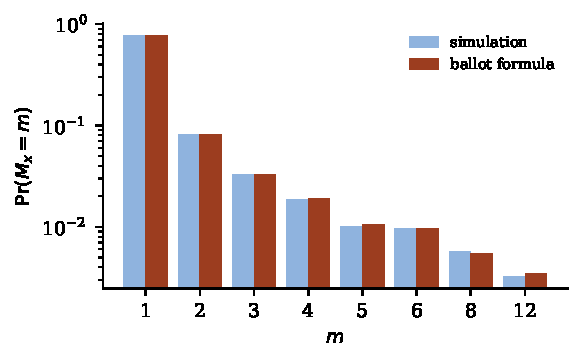
\includegraphics[width=0.8\textwidth]{figs/zeta_passage.pdf}
\caption{First passage law of the zeta subordinator ($\sigma=2$, $c=1/2$, $x=1$): simulation of $200000$ paths against the ballot formula of Theorem~\ref{thm:10dballot}.}\label{fig:10dpassage}
\end{figure}

\begin{proof}
By Proposition~\ref{prop:10dsublaw}, $\Prob(Z_t\in dx)\,dt = \sum_mp_t(m)\,\delta_{t/c-\log m}(dx)\,dt$ with $p_t(m) = d_t(m)m^{-\sigma}\zeta(\sigma)^{-t}$. On the line $\{t = c(x+\log m)\}$, parametrised by $x$, the measure $\delta_{t/c-\log m}(dx)\,dt$ is $c\,dx$. On the other side, $\Prob(\tau_x\in dt)\,dx = \sum_m\Prob(M_x = m)\,\delta_{c(x+\log m)}(dt)\,dx$. Distinct $m$ give disjoint lines, so \eqref{eq:10dkendall} gives $t\,\Prob(M_x = m) = x\,c\,p_t(m)$ with $t = c(x+\log m)$, which is the formula. The Laplace transform identity is $\E e^{-q\tau_x} = e^{-x\Phi(q)}$ written out. Finally $\psi'(0+) = 1/c+\zeta'/\zeta(\sigma)$; if it is nonnegative, $\Phi(0) = 0$ and $\Prob(\tau_x<\infty) = e^{-x\Phi(0)} = 1$.
\end{proof}

The theorem is a Lagrange inversion for Dirichlet series: summing over $m$ at $q = 0$ gives $\sum_m\frac x{x+\log m}d_{c(x+\log m)}(m)m^{-\sigma}\zeta(\sigma)^{-c(x+\log m)} = 1$ under the drift condition. We simulated $200000$ paths with $\sigma = 2$, $c = 0.5$, $x = 1$ (so $1/c = 2>-\zeta'/\zeta(2) = 0.5700$) and compared with the formula (Figure~\ref{fig:10dpassage}):

\begin{center}\small
\begin{tabular}{lcccccc}
\toprule
$m$ & $1$ & $2$ & $3$ & $4$ & $6$ & $12$\\
\midrule
simulation & $0.78075$ & $0.08160$ & $0.03273$ & $0.01873$ & $0.00970$ & $0.00324$\\
Theorem~\ref{thm:10dballot} & $0.77970$ & $0.08202$ & $0.03296$ & $0.01892$ & $0.00968$ & $0.00349$\\
\bottomrule
\end{tabular}
\end{center}

\noindent All differences are within two standard errors.

The construction needs only that $\log L$ has nonnegative Dirichlet coefficients, so it applies verbatim to a Dedekind zeta function $\zeta_K$, with values in $\{\log\mathrm N\mathfrak a\}$, and to $L(s,\pi\times\tilde\pi)$, partial or complete (Theorem~\ref{thm:ch09rs} and the paragraph after it), whose subordinator is the probabilistic object attached to $\pi$ to the right of $1$. It fails for $L(s,\chi)$ when $\chi$ takes the value $-1$ and for $L(s,\Delta)$, whose L\'evy measures are signed as in~\eqref{eq:ch09signed}: at $t=1$ the candidate weights $\chi(m)m^{-\sigma}/L(\sigma,\chi)$ take negative values, and even $L(s,\chi)L(s,\bar\chi)$, whose coefficient at $p^k$ is $2\operatorname{Re}\chi(p)^k/k$, does not suffice.\index{Kendall's identity}\index{ballot theorem}

\section{The Patie class}\index{Patie class}\index{Bernstein gamma function}

Patie and Savov \cite{patiesavov2018} introduced \emph{Bernstein gamma functions}: for a Bernstein function $\phi$, $W_\phi$ is the unique solution, in a suitable class, of
\[
W_\phi(z+1) = \phi(z)W_\phi(z),\qquad W_\phi(1) = 1,
\]
so that $W_\phi(n+1) = \phi(1)\cdots\phi(n)$ and $W_\phi = \Gamma$ for $\phi(z) = z$. They govern exponential functionals of L\'evy processes: for a subordinator $\eta$ with Laplace exponent $\phi$, the exponential functional $I_\phi = \int_0^\infty e^{-\eta_t}dt$ has $\E I_\phi^{\,n} = n!/W_\phi(n+1)$, and Patie and Savov extend this to the Mellin transform, $\E I_\phi^{\,z-1} = \Gamma(z)/W_\phi(z)$. Konstantopoulos, Patie and Sarkar use them to build a new class of van Dantzig solutions. Let $\Psi$ be the Laplace exponent of a possibly killed spectrally negative L\'evy process,
\[
\Psi(u) = -\kappa+au+\tfrac12\sigma^2u^2-\int_0^\infty\bigl(1-e^{-ur}-ur\mathrm{1}_{\{r<1\}}\bigr)\Pi(dr),
\]
with $\kappa\ge0$, $\sigma^2\ge0$, $\int_0^\infty\min(1,r^2)\,\Pi(dr)<\infty$, excluding the degenerate case in which the process is the negative of a subordinator, and with $\Psi(\frac12)\ge0$ (equivalently, the largest zero of $\Psi$ in $[0,\infty)$ lies in $[0,\frac12]$). Put
\[
J_\Psi(t) = \sum_{n\ge0}\frac{(-1)^nt^{2n}}{W_\Psi(n+1)},\qquad W_\Psi(n+1) = \Psi(1)\cdots\Psi(n),\qquad\mathcal D_P = \{J_\Psi\}.
\]

\begin{theorem}[Konstantopoulos, Patie and Sarkar \cite{konstantopoulospatiesarkar2024}, Theorem~4.1 and Lemma~5.7]\label{thm:10dpatie}
$\mathcal D_P\subset\mathcal D$. The partner $1/J_\Psi(i\cdot)$ is the characteristic function of $D_\Psi = \sqrt2\,B_{T_\Psi}$, where $B$ is a Brownian motion and $T_\Psi$ an independent positive self decomposable variable. The Bessel functions of \eqref{eq:10dbeta} are the case $\Psi(u) = u(u+\nu)$, up to the scaling $t\mapsto2t$.
\end{theorem}

They leave open whether $t\mapsto\xi(\frac12+it)/\xi(\frac12)$ lies in $\mathcal D_P$, noting that the question does not seem straightforward. We give a necessary condition that can be tested from Taylor coefficients.

\begin{proposition}[this book]\label{prop:10dpatietest}
Let $\Xi_\pi(z) = \sum_{n\ge0}a_nz^{2n}$ with all $a_n>0$, and suppose $\Xi_\pi(it)/\Xi_\pi(0) = J_\Psi(t)$ for some $\Psi$ as above. Then $\Psi(n) = a_{n-1}/a_n$ for $n\ge1$, and the sequence $\delta_n = \Psi(n+2)-2\Psi(n+1)+\Psi(n)$ is completely monotone in the sense of Hausdorff:
\[
(-1)^k\Delta^k\delta_n\ge0\qquad\text{for all }k\ge0,\ n\ge1,
\]
where $\Delta\delta_n = \delta_{n+1}-\delta_n$.
\end{proposition}

\begin{proof}
Comparing coefficients of $t^{2n}$ in $\sum(-1)^na_nt^{2n}/a_0$ and $J_\Psi(t)$ gives $W_\Psi(n+1) = a_0/a_n$, so $\Psi(n) = W_\Psi(n+1)/W_\Psi(n) = a_{n-1}/a_n$. For $u>0$ differentiation under the integral, justified by $\int\min(1,r^2)\Pi(dr)<\infty$ and the bound $r^2e^{-ur}\le C_u\min(1,r^2)$, gives $\Psi''(u) = \sigma^2+\int_0^\infty r^2e^{-ur}\Pi(dr)$. Hence
\[
\delta_n = \int_0^1\!\!\int_0^1\Psi''(n+u+v)\,du\,dv = \sigma^2+\int_0^\infty e^{-nr}(1-e^{-r})^2\,\Pi(dr),
\]
which is $\int_{[0,1]}y^n\,\rho(dy)$, where $\rho$ is the image of $(1-e^{-r})^2\Pi(dr)$ under $y = e^{-r}$ plus the atom $\sigma^2\delta_1$, a finite positive measure because $(1-e^{-r})^2\le\min(1,r^2)$. Then $(-1)^k\Delta^k\delta_n = \int y^n(1-y)^k\rho(dy)\ge0$.
\end{proof}

\begin{table}[t]
\centering\footnotesize
\setlength{\tabcolsep}{2.5pt}
\begin{tabular}{lrrrrrl}
\toprule
completed $L$ function & $d$ & $N$ & $\Psi(1)$ & $\Psi(2)$ & $\Psi(3)$ & Hausdorff test\\
\midrule
$\xi$ & 1 & 1 & 43.2807 & 93.0400 & 148.3165 & no violation, $k\le30$\\
$L(s,\chi_{-4})$ & 1 & 4 & 12.8181 & 30.2532 & 51.2721 & no violation, $k\le30$\\
$\Delta$ & 2 & 1 & 17.8012 & 38.0083 & 60.2084 & no violation, $k\le30$\\
$L(s,\chi_{-3})$ & 1 & 3 & 17.6363 & 39.5190 & 65.1347 & fails: $k=5$, $n=1$, $-1.24\cdot10^{-3}$\\
$L(s,\chi_5)$ & 1 & 5 & 12.7458 & 28.8566 & 47.9351 & fails: $k=7$, $n=3$, $-2.57\cdot10^{-6}$\\
11a1 & 2 & 11 & 7.8377 & 16.7656 & 26.6952 & fails: $k=10$, $n=11$, $-1.04\cdot10^{-9}$\\
$L(\chi_{-4})L(\chi_5)$ & 2 & 20 & 6.3909 & 13.7035 & 21.8976 & fails: $k=3$, $n=1$, $-2.92\cdot10^{-3}$\\
$\Sym^2$ 11a1 & 3 & 121 & 3.1133 & 6.7475 & 10.8728 & fails: $k=3$, $n=1$, $-1.75\cdot10^{-3}$\\
$\Sym^2$ 37a1 & 3 & 1369 & 1.4173 & 3.2542 & 5.4717 & fails: $k=3$, $n=2$, $-1.02\cdot10^{-4}$\\
Artin, $x^3-x-1$ & 2 & 23 & 5.8724 & 12.7516 & 20.5318 & no violation, $k\le8$\\
$\xi_K$, $K = \Q(x^3-x-1)$ & 3 & 23 & 5.1708 & 11.0277 & 17.4859 & no violation, $k\le8$\\
$L(\chi_5)L(\chi_{13})$ & 2 & 65 & 3.5773 & 8.4558 & 14.1903 & no violation, $k\le8$\\
$\Sym^3$ 11a1 & 4 & 1331 & 1.5923 & 3.6011 & 5.9504 & no violation, $k\le8$\\
$\Sym^4$ 11a1 & 5 & 14641 & 0.8871 & 2.1710 & 3.7238 & no violation, $k\le8$\\
\bottomrule
\end{tabular}
\caption{The Patie test of Proposition~\ref{prop:10dpatietest}: implied $\Psi(n) = a_{n-1}/a_n$ and the first violation of $(-1)^k\Delta^k\delta_n\ge0$, with order $k$, index $n$ and value. Computed from central Taylor coefficients with $150$ to $500$ digit arithmetic.}\label{tab:10dpatie}
\end{table}

We ran the test on the self dual completions of Table~\ref{tab:10dpatie}, using central Taylor coefficients computed for this book with PARI/GP at $150$ to $500$ digits. For $\xi$, $\Delta$ and $L(s,\chi_{-4})$ we used $40$ coefficients, which reach order $k = 30$; results are identical at $350$ and $500$ digits, and there is no violation. The minima over $n$ for $\xi$ are $2.01$, $1.79\cdot10^{-2}$, $6.75\cdot10^{-4}$, $4.47\cdot10^{-5}$ for $k = 0,1,2,3$, $1.90\cdot10^{-12}$ at $k = 20$ and $2.33\cdot10^{-10}$ at $k = 30$. This is evidence, not proof, on the question of Konstantopoulos, Patie and Sarkar. In six other cases the test fails decisively, with the violation stable under an increase of precision (for 11a1 identical at $350$ and $500$ digits, for $\Sym^2$ 11a1 at $150$ and $300$): \emph{these completed $L$ functions are not in $\mathcal D_P$}, up to the reliability of uncertified high precision arithmetic. The implied exponents of $\xi$ are $\Psi(1),\dots,\Psi(5) = 43.2807$, $93.0400$, $148.3165$, $208.4940$, $273.1404$, and of $\Delta$ are $17.8012$, $38.0083$, $60.2084$, $84.1425$, $109.6331$. No simple pattern by Gamma factor emerges: $L(s,\chi_{-4})$ passes while $L(s,\chi_{-3})$, with the same Gamma factor, fails. Figure~\ref{fig:10dpatie} shows the minima against $k$.

\begin{figure}[t]
\centering
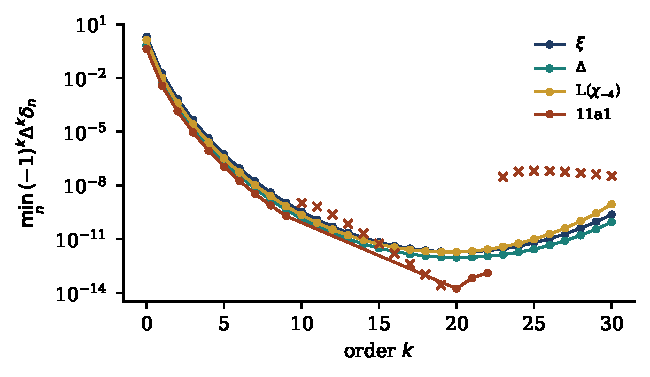
\includegraphics[width=0.78\textwidth]{figs/patie_test.pdf}
\caption{$\min_n(-1)^k\Delta^k\delta_n$ against the order $k$ for $\xi$, $\Delta$, $L(s,\chi_{-4})$ (no violation through $k=30$) and 11a1 (crosses: absolute values of negative minima, from $k = 10$).}\label{fig:10dpatie}
\end{figure}

Figure~\ref{fig:10dpatieheat} shows the whole table rather than its minima: for $\xi$ every entry of $(-1)^k\Delta^k\delta_n$ is positive, while for 11a1 a negative region opens from order $k=10$.

\begin{figure}[ht]\centering
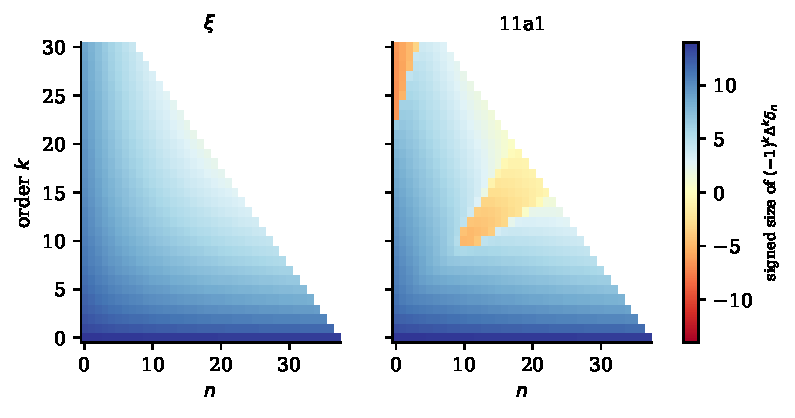
\includegraphics[width=0.95\textwidth]{figs/patie_heatmap.pdf}
\caption{Signed size of $(-1)^k\Delta^k\delta_n$ (blue positive, red negative, logarithmic scale) for $\xi$ and for the elliptic curve 11a1, computed from 40 central Taylor coefficients at 350 digits.}\label{fig:10dpatieheat}
\end{figure}

By Theorem~\ref{thm:10dpatie}, if $\Xi_\pi(it)/\Xi_\pi(0) = J_\Psi$, the partner would be $\sqrt2B_T$ with $T$ self decomposable and $\E e^{-sT} = \Xi_\pi(0)/\Xi_\pi(\sqrt s)$. Under GRH this is consistent with Theorem~\ref{thm:10dvdp}, where $V_\pi = \sqrt{2Z_\pi}N$ and $Z_\pi$, a GGC, is self decomposable; for $\xi$, self decomposability of $T$ is the unconditional statement of \cite{polson2018vdp} quoted above. Membership would add a structure on the Taylor coefficients, the factorisation $a_0/a_n = \Psi(1)\cdots\Psi(n)$ through a L\'evy exponent. A representing $\Psi$ would have no Brownian component. Indeed $\Psi(u)/u^2\to\sigma^2/2$ for any such exponent, and if $\Psi(n)\ge\epsilon n^2$ for all large $n$ then $a_n\le Ca_0\epsilon^{-n}(n!)^{-2}$, so $|\Xi_\pi(z)|\le C'e^{2|z|/\sqrt\epsilon}$, contradicting the growth $\exp(cx\log x)$ of $\Xi_\pi(x)$ on the real axis forced by the Gamma factors; hence $\liminf\Psi(n)/n^2 = 0$ and $\sigma = 0$. For $\xi$ the ratios $\Psi(n)/n^2$ are $43.3$, $23.3$, $16.5$, $13.0$, $10.9$ for $n = 1,\dots,5$. Interpolating the $\Psi(n)$ by a Bernstein gamma type function is a well posed computational problem (Computational Problem~\ref{cp:10dpatie}).

\section{Notes}

The van Dantzig problem was posed in 1958 \cite{vandantzig1958}; Lukacs \cite{lukacs1968,lukacs1970} introduced the class we call $\mathcal D_L$ and the operators $L^{(p)}$, and Ostrovskii \cite{ostrovskii1970} constructed hyperbolic examples. Hinds \cite{hinds1974} studied the Gamma and symmetric Beta examples; for the latter see also \cite{amdeberhan2012,jurek2010,hasebesimonwang2018}, and for Bessel hitting times Kent \cite{kent1978}. Thorin \cite{thorin1977} introduced generalized gamma convolutions and Bondesson \cite{bondesson1992} developed them, including the extended class. Biane, Pitman and Yor \cite{bpy2001} gave the Brownian reading of $\xi$, and Biane \cite{biane2009} the matrix Brownian reading of P\'olya's Macdonald function theorem \cite{polya1926}. Wald couples with infinitely divisible members are due to Roynette and Yor \cite{roynetteyor2005}, building on Hartman's theorem on the reciprocal Gamma function \cite{hartman1976}; they also rewrote the Riemann hypothesis through Wald couples and P\'olya frequency functions (their Th\'eor\`eme~V.3.2) and observed that the P\'olya variable of $\xi$ is not infinitely divisible. The equivalence between Hadamard factorisation, van Dantzig pairs, Wald couples and Thorin's condition, the $2\sin^2$ lemma, the transport of Euler product L\'evy measures, and the shifted Thorin representations of $\xi$ are from the first author \cite{polson2017,polson2018vdp}. Konstantopoulos, Patie and Sarkar \cite{konstantopoulospatiesarkar2024} proved the Lukacs class characterisation of the Riemann hypothesis and of the Lee Yang property \cite{leeyang1952,newman1974,newmanwu2020}, and introduced $\mathcal D_P$ through the Bernstein gamma functions of Patie and Savov \cite{patiesavov2018}. The positivity criterion for $\xi$ is due to Hinkkanen \cite{hinkkanen1997} and Lagarias \cite{lagarias1999}; Weil's explicit formula \cite{weil1952} is used in the form of \cite{iwanieckowalski2004}. Kendall's identity is from \cite{kendall1957}, the ballot theorem from Tak\'acs \cite{takacs1967}, and fluctuation theory of spectrally negative processes from \cite{bertoin1996,kyprianou2014}. Ours are Theorem~\ref{thm:10dvdp} and Theorem~\ref{thm:10dshift} in the generality of Chapter~\ref{ch:10b} (for $\zeta$ they are due to the authors cited above), Proposition~\ref{prop:10dsmooth}, the Thorin density $u_\Gamma$ in \eqref{eq:10dnewman}, Proposition~\ref{prop:10dsublaw}, Theorem~\ref{thm:10dballot}, Proposition~\ref{prop:10dpatietest} and all computations; each is an elementary consequence of the cited results, and none proves a Riemann hypothesis.

\section{Exercises}

\begin{enumerate}
\item Verify that $\frac2{\sqrt\pi}e^{x-e^{2x}}$ is a probability density with characteristic function $\frac1{\sqrt\pi}\Gamma(\frac{1+is}2)$, and prove $|\Gamma(\frac{1+is}2)|^2 = \pi/\cosh(\pi s/2)$. Show that $t\mapsto\sqrt\pi/\Gamma(\frac{1-t}2)$ takes the values $-\frac12$ at $t=2$ and $2$ at $t=-2$, so that it is neither even nor bounded by $1$; deduce that the Hinds law is not in $\mathcal D$, while the product is.
\item\label{ex:10dbeta} For $\nu>-\frac12$ expand $\cos(sx)$ and use Beta integrals to show that the symmetric Beta law of density $(1-x^2)^{\nu-1/2}/B(\nu+\frac12,\frac12)$ has characteristic function $\Gamma(\nu+1)(s/2)^{-\nu}J_\nu(s)$. Identify the cases $\nu = 0,\frac12,1$, and the limit $\nu\downarrow-\frac12$.
\item Prove the Laplace pair $\int_0^\infty e^{-yz}\cos(2\sqrt{az})(\pi z)^{-1/2}dz = y^{-1/2}e^{-a/y}$ and deduce \eqref{eq:10dpair}. Then, for $f(w) = w^2+\gamma^2$ at $\alpha = \epsilon$, where $\nu$ is a signed measure, check directly that the two expressions in \eqref{eq:10dU} agree, recovering the single zero case of Proposition~\ref{prop:10dsmooth}.
\item Show that $d_1 = 1$ and that $d_2$ is the divisor function. For $\sigma>1$ and $t>0$ compute $\E X_t$ and $\operatorname{Var}X_t$ in terms of $\zeta'/\zeta$ and its derivative, and check the first entry $\Prob(M_1 = 1) = \zeta(2)^{-1/2}\cdot1 = 0.77970$ of the table for $\sigma = 2$, $c = \frac12$.
\item\label{ex:10dnotid} Show that the characteristic function of an infinitely divisible law has no real zero. (If $\varphi = \varphi_n^n$ for every $n$, then $|\varphi_n|^2 = |\varphi|^{2/n}$ converges to the indicator of $\{\varphi\ne0\}$, which is therefore continuous at $0$ and a characteristic function, hence identically $1$.) Deduce that $W_\zeta$ and $W_\Delta$ are not infinitely divisible (Remark~\ref{rem:10dnotid}).
\item For $\cos t$ show that the Patie test of Proposition~\ref{prop:10dpatietest} gives $\Psi(n) = 2n(2n-1)$, the exponent $\Psi(u) = 4u^2-2u$ of Brownian motion with variance $8$ and drift $-2$, with largest zero $\frac12$, and that $\delta_n = 8$. Do the same for $\sin t/t$ and for $f_\nu$ of \eqref{eq:10dbeta}, and compare with Theorem~\ref{thm:10dpatie}.
\end{enumerate}

\section{Open computational problems}

\begin{compproblem}[Certified Patie test and Bernstein gamma interpolation]\label{cp:10dpatie}
Objective: certify the Hausdorff inequalities of Proposition~\ref{prop:10dpatietest} for $\xi$, $\Delta$ and $L(s,\chi_{-4})$ through order $k = 100$, and attempt to reconstruct $\Psi$. Objects and scale: the first $120$ central Taylor coefficients of each completed function. Route: coefficients in rigorous ball arithmetic (Arb, cross checked with PARI/GP \texttt{lfunlambda} at $2000$ digits), interval finite differences, then a least squares fit of $\Psi(u) = au+\int(e^{-ur}-1+ur\mathrm{1}_{\{r<1\}})\Pi(dr)$ with $\Pi$ a positive combination of $r^{-1-\beta}e^{-\lambda r}$, via the Bernstein gamma recursion of \cite{patiesavov2018}. Deliverable: certified lower bounds for $\min_n(-1)^k\Delta^k\delta_n$, the first certified violation if any, and the fitted L\'evy measure with residuals. Why it matters: a certified violation answers the question of Konstantopoulos, Patie and Sarkar negatively for $\xi$; a stable fit suggests a candidate Brownian subordination structure for the partner of $\xi$.
\end{compproblem}

\begin{compproblem}[Transported Thorin densities in the strip]
Objective: map the sign of the total transported density $V_a$ of Theorem~\ref{thm:10dshift}, and of its arithmetic and archimedean parts, for basepoints $\alpha = \frac12+a\in(\frac12,1]$. Objects and scale: $\xi$, $\Delta$ and $L(s,\chi_{-4})$, $a\in\{0.01,0.02,\dots,0.5\}$, $\sqrt z\le10^4$; the arithmetic part from all primes below $10^9$ with smoothing. Route: PARI/GP \texttt{lfunlambda} derivatives on GPU grids; interval arithmetic near the minima. Deliverable: the region of the $(a,z)$ plane where positivity is certified, the minimum of $V_a$ for each $a$, the location of the minima relative to the $\gamma_k^2$, and, for $\Lambda(s,\chi_{-4})$, the margin $\min_{t\ge1}\bigl(\operatorname{Re}\Lambda'/\Lambda(\alpha+it)-\Lambda'/\Lambda(\alpha)\bigr)$ in Theorem~\ref{beta:thm:minall}. Why it matters: by the argument of Theorem~\ref{thm:10dshift}(iv), certified positivity of $V_{a'}$ on $\sqrt z\le T$ for every $a'\ge a$ (interval arithmetic in $a'$ as well as in $z$) excludes zeros with real part above $\frac12+a$ and height at most $T$, so the map is a Thorin form of zero free region computations.
\end{compproblem}

\begin{compproblem}[First passage tables and large deviations for Euler subordinators]
Objective: tabulate the first passage laws of Theorem~\ref{thm:10dballot} and their large deviations. Objects and scale: $\zeta$, $\zeta_K$ for the $100$ quadratic and cubic fields of smallest discriminant, and the Rankin Selberg functions $L(s,\pi\times\tilde\pi)$, partial or complete, for the eleven functions of Table~\ref{tab:10bcatalogue}; $\sigma\in\{1.1,1.5,2\}$, $x\le50$, $m\le10^8$. Route: generalized divisor functions by sieving, $\Phi$ by Newton iteration on $\psi$, Monte Carlo with $10^7$ paths. Deliverable: tables of $\Prob(M_x = m)$, verification of $\sum_m\Prob(M_x=m) = 1$ to $10^{-10}$, and the rate function $\lim x^{-1}\log\Prob(\tau_x>\theta x)$ compared with the Legendre transform of $\psi$. Why it matters: these are the probabilistic objects attached to $\pi$ to the right of $1$, and their behaviour as $\sigma\downarrow1$ is governed by the pole and the zero free region of $L(s,\pi\times\tilde\pi)$.
\end{compproblem}

\begin{compproblem}[Van Dantzig and P\'olya frequency tests across LMFDB]
Objective: test numerically, without zeros, whether the partner $\Xi_\pi(0)/\Xi_\pi(t)$ is the characteristic function of a P\'olya frequency density. Objects and scale: all self dual $L$ functions in LMFDB of degree at most $4$ and conductor below $10^4$, whether or not the P\'olya kernel is positive. Route: evaluate $\Xi_\pi(t)$ on $|t|\le200$ with PARI/GP, invert the Fourier transform by quadrature with error control, and compute Toeplitz determinants $\det[g(x_i-y_j)]$ of orders $2$ to $6$ on random grids. Deliverable: for each function the minimum density, the smallest Toeplitz minor found, and a table of failures with diagnosis (quadrature error or genuine). Why it matters: by Theorem~\ref{thm:10dvdp} the P\'olya frequency property of $V_\pi$ is equivalent to GRH, and log concavity, observed here for $\Delta$, is its first rung.
\end{compproblem}
